\documentclass{article}
\usepackage[utf8]{inputenc}
\usepackage[portuges]{babel}
\usepackage{ntheorem}
\usepackage{amsfonts}
\usepackage{amsmath}
\usepackage{float}
\usepackage{amssymb}
\usepackage{mathtools}

\usepackage{multicol}
\theorembodyfont{\upshape}
\theoremseparator{.}
\newtheorem{ex}{Exercício}[section]
\newtheorem*{defn}{Definição}

\usepackage{enumitem}
\setlist[enumerate, 1]{label=\alph*)}
\setlist[enumerate, 2]{label=(\roman*)}

\usepackage{listings}
\lstset{basicstyle=\ttfamily,mathescape,keepspaces,tabsize=2,
literate=
  {á}{{\'a}}1
  {à}{{\`a}}1
  {ã}{{\~a}}1
  {é}{{\'e}}1
  {ê}{{\^e}}1
  {í}{{\'i}}1
  {ó}{{\'o}}1
  {ú}{{\'u}}1
  {ç}{{\c{c}}}1}
\usepackage{graphicx}
\usepackage{xcolor}
\usepackage{url}

\title{Projeto de ME - Segunda Entrega}
\author{Juha Videman, Duarte Maia, Maria Madrugo}
\date{Data de entrega: 4 de fevereiro de 2022}
\setlength{\parindent}{0pt}
\newcommand{\Z}{\mathbb{Z}}
\newcommand{\R}{\mathbb{R}}
\usepackage[margin=0.9in]{geometry}
\newcommand{\N}{\mathbb{N}}
\newcommand{\Q}{\mathbb{Q}}

\begin{document}

\noindent {\bf Unidade de Ensino de Matemática Aplicada e Análise Numérica}

\noindent Departamento de  Matemática/Instituto Superior
Técnico \vspace{3mm}

\noindent {{\bf Matem\'atica Experimental }} ({\small LMAC}) -- 2$^{\rm o}$ Período de 2021/2022

\bigskip

\begin{center}
{\bf\Large   Trabalho Computacional}\\ 
\smallskip
{\large Segunda Entrega}\\
Data de entrega: 4 de Fevereiro de 2022
\end{center}

\bigskip
\hrule

\section*{Introdução e Instruções [Novo]}

Instruções de entrega: Cada grupo deverá entregar um notebook \textit{Mathematica} e um relatório em pdf para o e-mail \texttt{jvideman@math.tecnico.ulisboa.pt}. O relatório deverá conter as respostas às questões, e o notebook deverá conter o código utilizado para as responder. Podem elaborar o relatório em Word, Mathematica ou Latex, desde que o submetam em pdf. Se quiserem usar Latex podem pedir um template ao professor. Se algum código demorar algum tempo a correr, devem indicá-lo, preferencialmente no notebook,  com um comentário a indicar a estimativa de tempo. \texttt{(* Isto é um exemplo de um comentário. Este texto não é executado pelo processador do Mathematica.*)}

\smallskip

Critérios de avaliação: Os trabalhos serão cotados com base nas respostas aos exercícios. Não será avaliada a qualidade do código no notebook \textit{Mathematica}, mas o código será lido e executado para garantir que coincide com as repostas dadas no relatório e que o raciocínio está correto. Como tal, a questão à qual cada pedaço de código está associado deverá ser indicada com um comentário. A qualidade do relatório, no entanto, será avaliada, pelo que deve estar sucinto, claro, bem-escrito e bem-organizado. \textbf{Em adição,} o relatório deverá ser autosuficiente (isto é, conter todas as imagens e outputs relevantes) e deverá conter explicação para as partes do código mais elaboradas. 

\smallskip

A não ser que indicado \emph{explicitamente} em contrário, justificações analíticas não são necessárias. Por exemplo, para justificar que uma função é contínua seria apenas necessário fazer o gráfico e apontar que não há descontinuidades.

\section{O Crivo de Sundaram [3 valores]}

Nas aulas teóricas, o aluno terá aprendido sobre o crivo de Eratóstenes, que é um algoritmo para determinar todos os números primos até um dado $n$ natural. Neste exercício, vai implementar e estudar outro crivo, chamado o crivo de Sundaram.

O algoritmo é o seguinte:
\begin{lstlisting}[columns=fullflexible]
Seja $L = \mathtt{Range[n]}$;
Seja $i = 1$;
Enquanto $\color{red}2 i (i+1)\color{black} \leq n$;
	Se $L[[i]] \neq \mathtt{"REMOVIDO"}$;
		Seja $j = 3i + 1$;
		Enquanto $j \leq n$:
			$L[[j]] \leftarrow \mathtt{"REMOVIDO"}$;
			$j \leftarrow j + 2i + 1$
	$i \leftarrow i+1$
Seja $out$ uma lista vazia;
Para cada elemento $x \in L$;
	Se $x \neq \mathtt{"REMOVIDO"}$;
		Adicionar $2x+1$ a out
Retornar $out$.
\end{lstlisting}

\begin{ex}
Implemente o crivo de Sundaram em Mathematica, criando uma função \texttt{sundaram[n]}. Teste-o para vários valores de $n \in \Z^+$. Explique, com base nos seus testes, o que o crivo retorna.
\end{ex}


\begin{ex}
Defina a função \texttt{sundquot[n\_] := Length[sundaram[n]] Log[n] / n}. Justifique que o limite, quando $n$ vai para infinito, de \texttt{sundquot[n]}, existe e calcule-o, justificando com a matéria dada nas aulas. Calcule \texttt{sundquot[n]} para $n = 10^i, i = 1, \dots, 7$. Compare o resultado com o limite esperado e comente.
\end{ex}

\begin{ex}
O objetivo deste exercício é estimar a redundância do crivo de Sundaram. Defina uma função \texttt{redundancia[n]} que executa o crivo de Sundaram para $n$ e retorna o número de vezes que o código remove um número que foi previamente removido.

Verifique o seu código, comparando os seus resultados com os da tabela seguinte:


\begin{center}
\begin{tabular}{r|lllll}
\texttt{n} & 10 & 20 & 30 & 40 & 50 \\
\hline
\texttt{redundancia[n]} & 0 & 1 & 4 & 6 & 6 \\
\end{tabular}
\end{center}

Aplicando visualizações apropriadas, faça uma conjetura tão precisa quanto consiga relativamente ao comportamento assintótico de \texttt{redundancia[n]}. Por outras palavras, encontre uma expressão simples em função de $n$ que seja uma boa aproximação desta função para $n$ grande e justifique graficamente.
\end{ex}

\begin{ex}
Justifique analíticamente o funcionamento do crivo de Sundaram, por comparação com o crivo de Eratóstenes.
\end{ex}

\section{Baralhos [3 valores]}

Neste exercício vai investigar uma forma de baralhar baralhos de cartas. Para este efeito, o conteúdo das cartas é irrelevante, pelo que basta representar as cartas por números de 1 a 52.

\begin{ex}
Considere o seguinte algoritmo para baralhar um baralho.

Um `riffle shuffle' consiste em partir o baralho ao meio e juntar as duas metades com as cartas a alternar. Por exemplo, dado um baralho cujas cartas são $c_1, c_2, \dots, c_{2n}$, o seu riffle shuffle é dado por
\[c_1, c_{n+1}, c_2, c_{n+2}, \dots, c_n, c_{2n}.\]

Se o baralho de cartas tiver um número ímpar de cartas, digamos $c_1, \dots, c_{2n+1}$, o seu riffle shuffle é dado por
\[c_1, c_{n+2}, \dots, c_n, c_{2n+1}, c_{n+1}.\]

Implemente uma função que recebe um baralho de cartas (ou seja, uma lista) e retorna o seu riffle shuffle.

\smallskip

Sugestão: Investigue o comando  \texttt{Riffle}.
\end{ex}

\begin{ex}
Apresentamos na figura \ref{shuffle8} uma visualização dos diversos riffle shuffles de um baralho de oito cartas, isto é: a $n$-ésima linha representa o baralho após $n$ riffle shuffles.

Como pode ver, após três shuffles o baralho volta à situação original. A figura \ref{shuffle52} mostra também o resultado de aplicar o riffle shuffle a um baralho de 52 cartas, e como pode perceber pela figura, o baralho volta à posição original após 8 shuffles.

Verifique estas afirmações. (Não é necessário reproduzir as imagens abaixo.)

\begin{figure}[H]
\centering
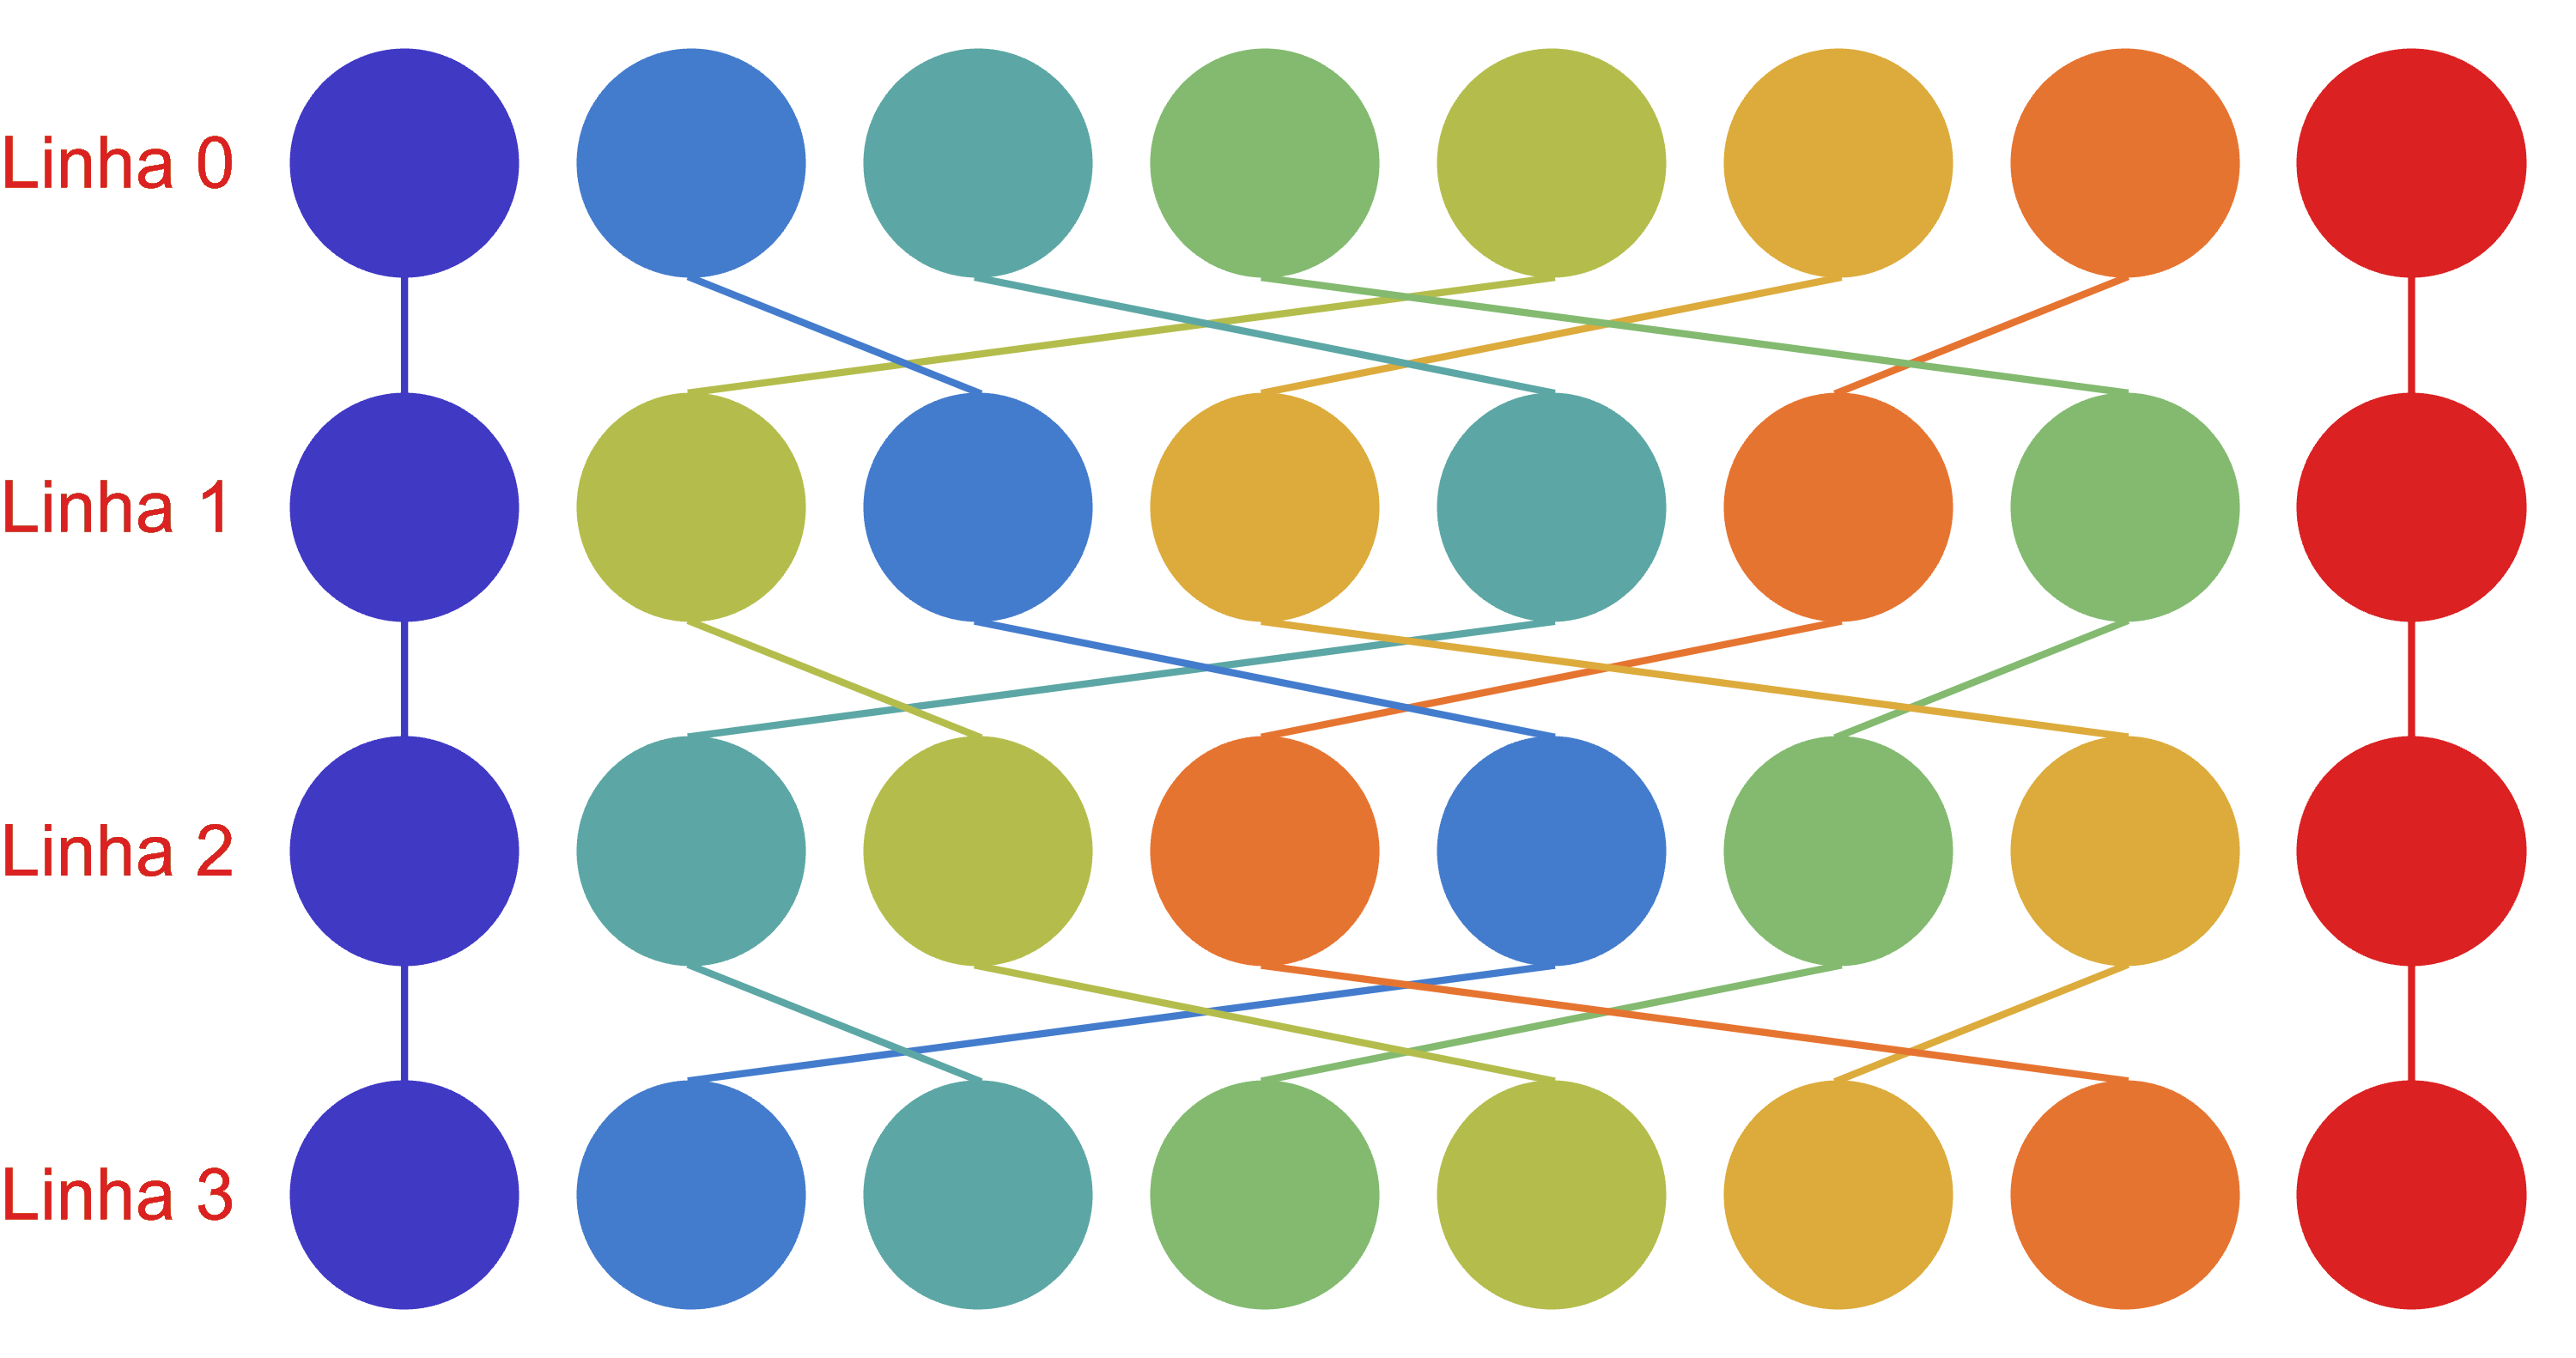
\includegraphics[width=.75\textwidth]{shuffle8}
\caption{Uma visualização das iterações do riffle shuffle num baralho com 8 cartas.}\label{shuffle8}
\end{figure}

\begin{figure}[H]
\centering
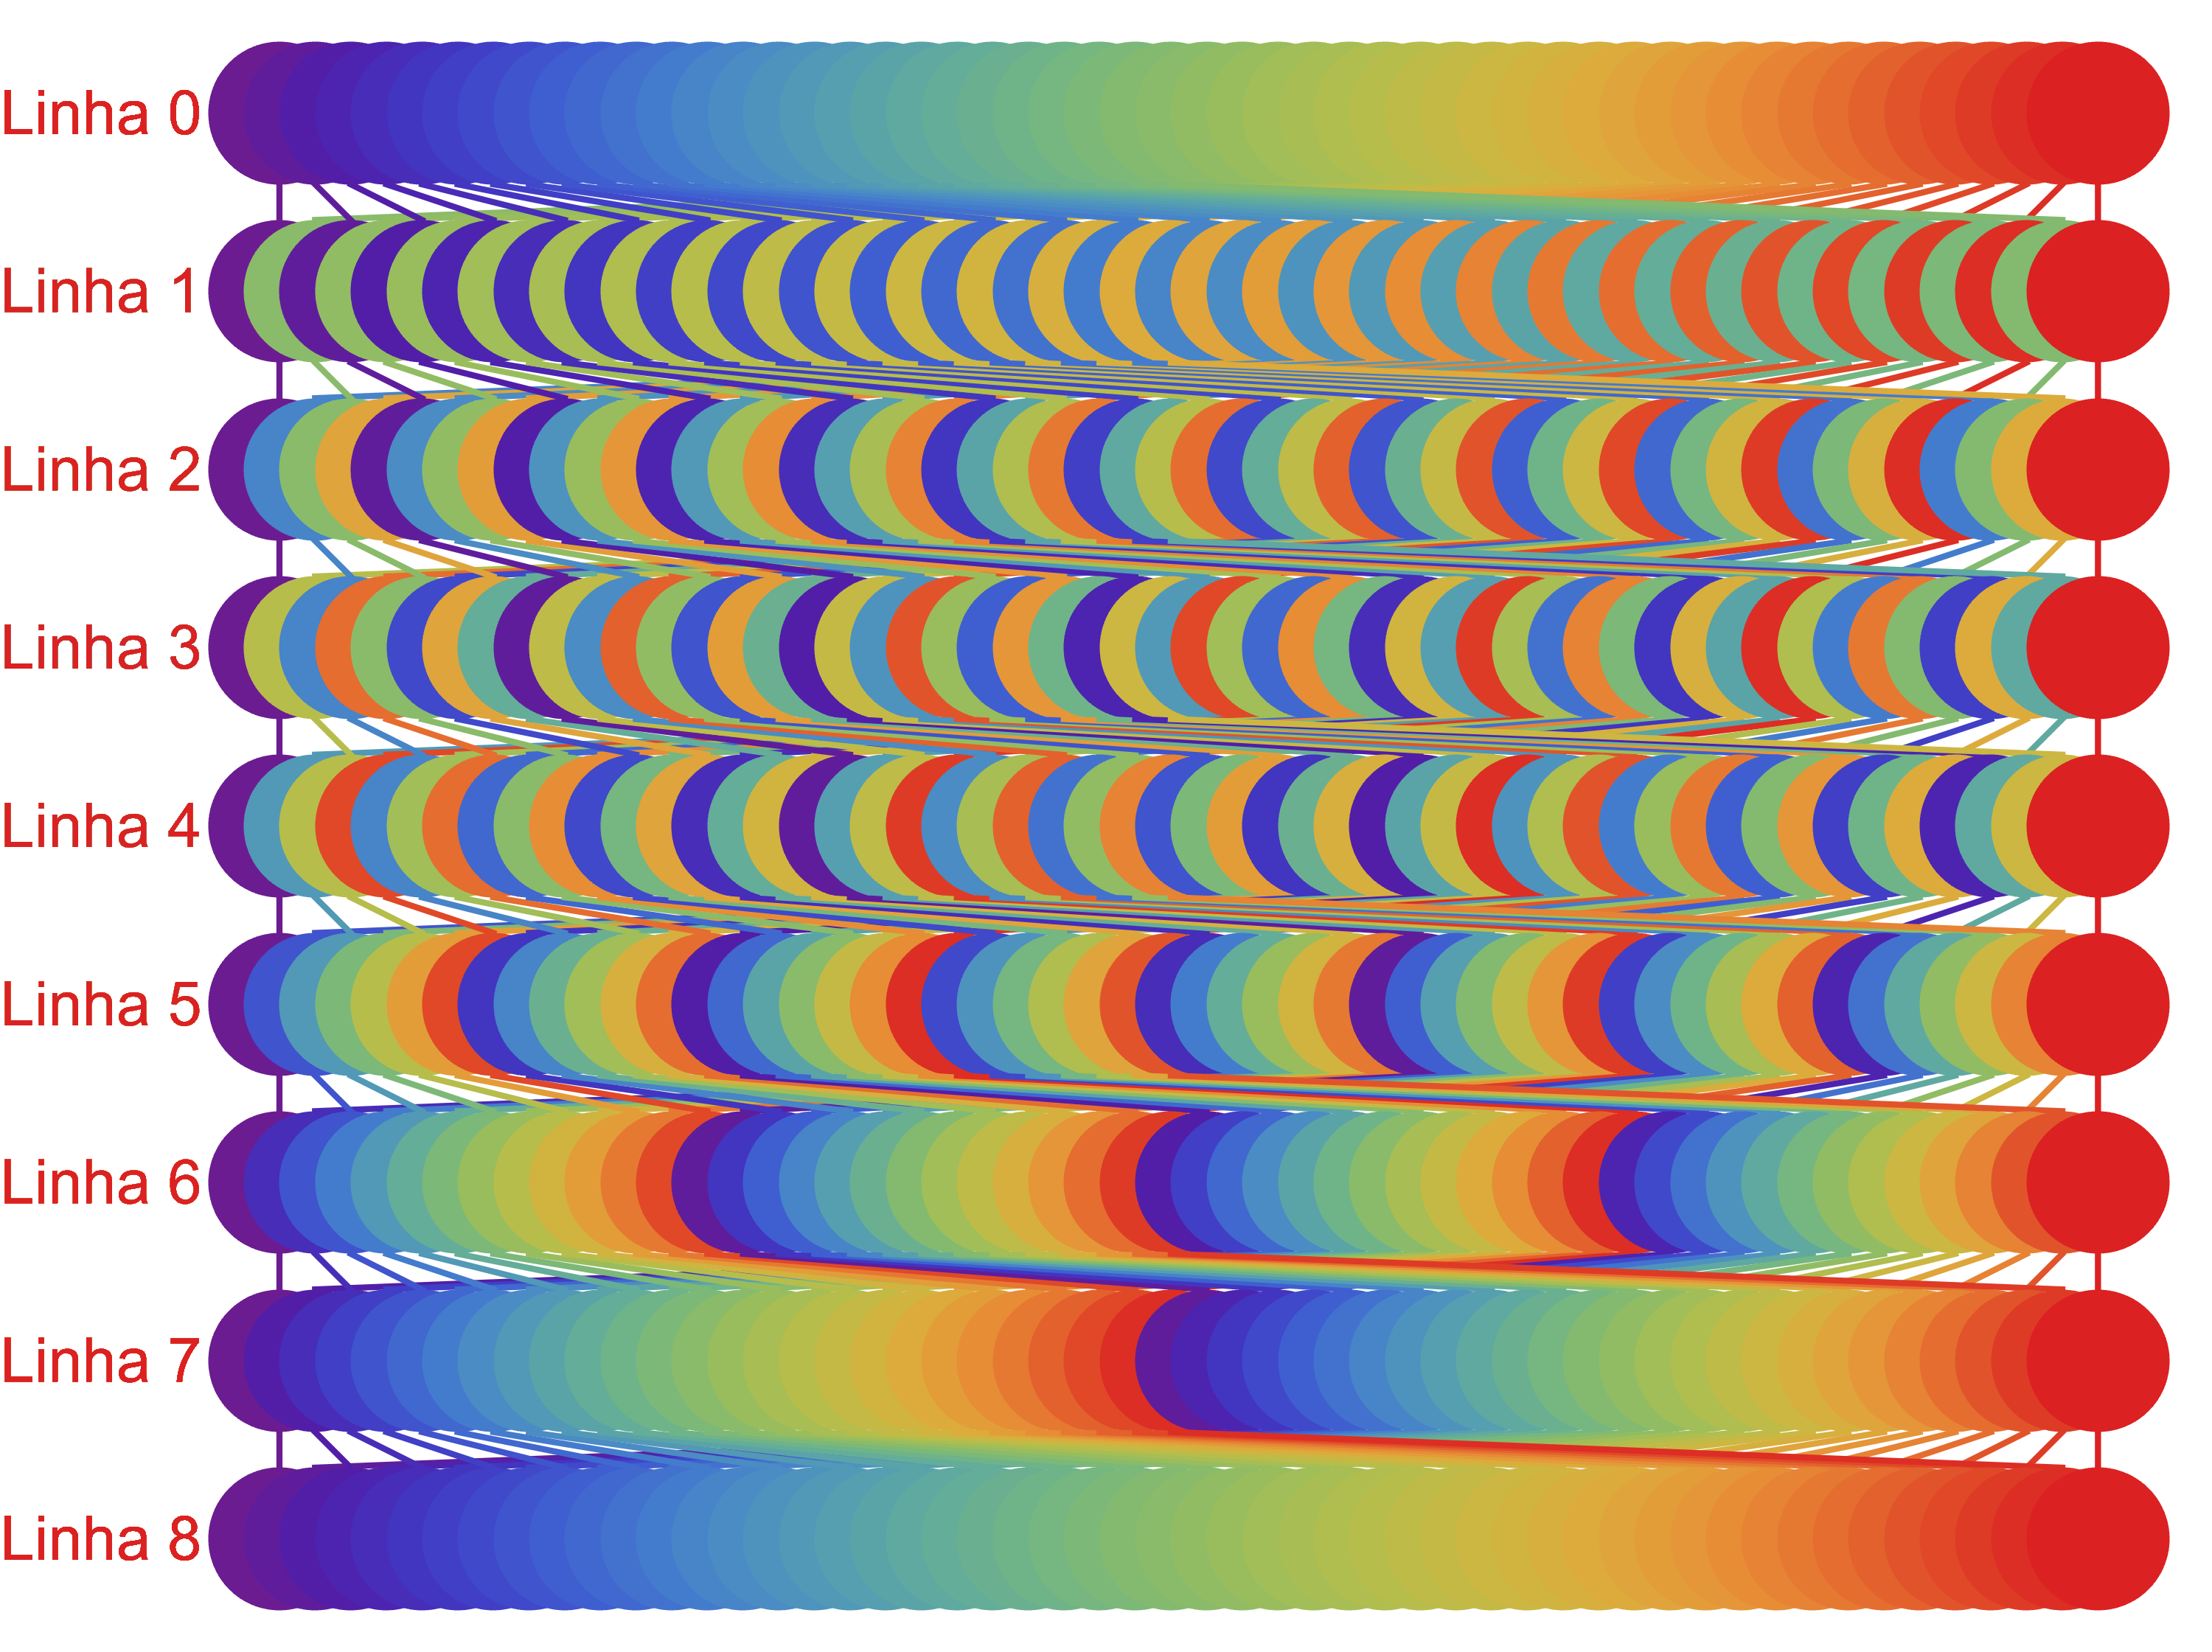
\includegraphics[width=.75\textwidth]{shuffle52}
\caption{Oito riffle shuffles de um baralho com 52 cartas.}\label{shuffle52}
\end{figure}
\end{ex}

\begin{ex}
Defina uma função \texttt{ord[n]} que, dado $n$, retorna o número de riffle shuffles necessários para um baralho com $n$ cartas retornar à posição original.

Use a função \texttt{DiscretePlot} para mostrar o gráfico dessa função para alguns valores de $n$. Use esse gráfico para formular uma conjetura que relacione os valores de \texttt{ord[n]} para $n$ par e ímpar.
\end{ex}

\begin{ex}
Faça um gráfico de \texttt{ord[n]} apenas com valores pares de $n$. Usando a função \texttt{Show}, sobreponha a este os gráficos de $y = x-2$ e $y = \frac{\log x}{\log2}$.

Formule uma conjetura que relacione estas três funções.
\end{ex}

\begin{ex}
Investigue os valores pares de $n$ tais que $\mathtt{ord[n]} = \frac{\log n}{\log 2}$. Quais são estes valores?
\end{ex}

\section{Fracções Contínuas Generalizadas [4 valores]}

Tal como se definem fracções continuas, é possível definir fracções continuas generalizadas associadas a $a=\{a_n\}_n$ e $b=\{b_n\}_n$ da seguinte forma:

$$b_0+\displaystyle{ \frac{a_1 }
{ b_1+\displaystyle{\frac{a_2}{ 
                           {\begin{array}{l}
                              b_2+\displaystyle{ \frac{a_3}{b_3+ \displaystyle \frac{a_4}{b_4+\ldots } }  }\,\, 
                           \end{array}
                           }
                           }}}} $$

\vspace{1mm}

\begin{ex}
Defina uma função que recebe duas listas $a=(a_1,\dots a_n)$ e $b=(b_0, \dots, b_n)$ calcula o número que corresponde à fracção continua generalizada finita associada a $a$ e $b$. 

Verifique computacionalmente que $$\ln 2 = \sum_{k=1}^{\infty} \frac{(-1)^{k-1}}{k}=\displaystyle{ \frac{1 }
{ 1+\displaystyle{\frac{1^2}{ 
                           {\begin{array}{l}
                              1+\displaystyle{ \frac{2^2}{1+ \displaystyle \frac{3^2}{1+\ldots } }  }\,\, 
                           \end{array}
                           }
                           }}}} $$
\end{ex}

\begin{ex}
Determine os números que correspondem às seguintes fracções continuas generalizadas:
  
\vspace{-1mm}  

   \[
\hspace{0.5cm}
2+
\displaystyle{ \frac{2 }
{ 2+\displaystyle{\frac{3}{ 
                           {\begin{array}{l}
                              3+\displaystyle{ \frac{4}{4+ \displaystyle \frac{5}{5+\ldots } }  }\,\, 
                           \end{array}
                           }
                           }}}} \qquad \qquad 
                              1+
\displaystyle{ \frac{2 }
{ 3+\displaystyle{\frac{1}{ 
                        {\begin{array}{l}
                              12+\displaystyle{ \frac{1}{20+ \displaystyle \frac{1}{28+\ldots } }  }\,\, 
                             \end{array}
                             }
                             }}}}      \qquad \qquad      
\displaystyle{ \frac{1 }
{ 2+\displaystyle{\frac{1^2}{ 
                          {\begin{array}{l}
                      6+\displaystyle{ \frac{2^2}{10+ \displaystyle \frac{3^2}{14+\ldots } }  }\,\, 
                        \end{array}
                         }
                          }}}}                                                   
\]

Sugestão: Considere as funções \texttt{Tan}, \texttt{ArcTan}, \texttt{Sqrt} e a constante \texttt{E}.
\end{ex}

\begin{ex}
Verifique que as seguintes fracções contínuas generalizadas convergem para $\pi$. Ordene as três frações contínuas em termos da sua rapidez de convergência.  

 \[
\hspace{0.5cm}
\displaystyle{ \frac{4 }
{ 1+\displaystyle{\frac{1^2}{ 
                           {\begin{array}{l}
                              2+\displaystyle{ \frac{3^2}{2+ \displaystyle \frac{5^5}{2+\ldots } }  }\,\, 
                           \end{array}
                           }
                           }}}} \qquad \qquad 
                              3+
\displaystyle{ \frac{1^2 }
{ 6+\displaystyle{\frac{3^2}{ 
                        {\begin{array}{l}
                              6+\displaystyle{ \frac{5^2}{6+ \displaystyle \frac{7^2}{6+\ldots } }  }\,\, 
                             \end{array}
                             }
                             }}}}      \qquad \qquad      
\displaystyle{ \frac{4 }
{ 1+\displaystyle{\frac{1^2}{ 
                          {\begin{array}{l}
                      3+\displaystyle{ \frac{2^2}{5+ \displaystyle \frac{3^2}{7+\ldots } }  }\,\, 
                        \end{array}
                         }
                          }}}}                                                   
\]
\end{ex}

\begin{ex}
Considere a equação $x^2+bx+c=0.$ Notando que esta condição implica $x=-b+\frac{-c}{x}$,
\begin{enumerate}
    \item Determine uma fracção continua generalizada candidata a representar uma solução da equação.
    \item Use a alínea anterior para aproximar soluções das equações $x^2-4x+4=0,$ $x^2-4x+2=0$ e $x^2-4x+6=0$ e comente os resultados.
    \item Considere $b=0$ e $c<0$. Note que, neste caso, resolver a equação corresponde a calcular $\sqrt{-c}$.
    \begin{enumerate}
        \item As aproximações da solução da equação convergem?
        \item Mostre que para qualquer $p\in \mathbb{R}^+$ $x+p=2p+\frac{-c-p^2}{x+p}$, e use esta equação para determinar aproximações de $\sqrt{-c}$. Aproxime $\sqrt{3}$, $\sqrt{4}$ e $\sqrt{5}$ usando este método. [Sugestão: Note que a equação é equivalente a $x^2-p^2=-c-p^2$.]
        \item Usando a alínea anterior, justifique que $\sqrt{n}=[r;\overline{2r}]$ se e só se $n=r^2+1$.
    \end{enumerate}
    
    \item O objetivo desta alínea é determinar, para $b \neq 0$, sob que condições se tem convergência da fração contínua generalizada acima para uma solução da equação $x^2 + bx + c = 0$.
    \begin{enumerate}
    \item Crie uma função que, dados $b$ e $c$, determina se a fração contínua converge para uma solução da equação, calculando uma iterada grande da fração contínua e verificando se esta é uma raiz aproximada de $x^2 + bx +c=0$. O seu programa deve retornar \texttt{Green} (comando de \texttt{Mathematica}) em caso afirmativo, \texttt{Red} em caso negativo e \texttt{Yellow} se $b = 0$. 
    
    Nota: Este método de determinar convergência é falível em princípio, mas é bom o suficiente para o propósito.
    
    \item Usando os comandos \texttt{Graphics} e \texttt{Point}, represente no plano uma grelha adequadamente densa de pontos $(b,c)$, com o ponto $(b,c)$ colorido de verde ou vermelho consoante o funcionamento do método.
    
    Usando o comando \texttt{Show}, sobreponha a figura anterior ao gráfico de uma função apropriada, de modo a determinar a condição que determina que pontos são verdes e quais são vermelhos.
    
    \item Conjeture sob que condições o método funciona. Comente a condição obtida.
    
    Nota: Não se esqueça de averiguar os casos críticos.
    \end{enumerate}
\end{enumerate}
\end{ex}

\section{O Problema de Frobenius [5 valores]}

Suponha que $a,b,n\in\mathbb{N}$ e considere a equação diofantina
\begin{equation}
ax+by=n \, .
\label{dio}
\end{equation}

Seja $g(a,b)$ o maior inteiro $n$ tal que a equação \eqref{dio} {\bf não} admite soluções inteiras não negativas.


\begin{ex}
Mostre analíticamente que $g(a,b)=\infty$ se  mdc($a,b)\neq 1$, isto é: existem inteiros $n$ arbitrariamente grandes tais que $ax + by = n$ não tem soluções inteiras não negativas.
\end{ex}

\begin{ex}
Calcule $g(a,b)$ para $2\leq a,b\leq 20$, mdc$(a,b)=1$, e, com base nos seus resultados, apresente uma fórmula para  $g(a,b)$ em função de $a$ e $b$.
\end{ex}


Seja $h(a,b)$ o número total de  inteiros positivos $n$ para os quais a equação \eqref{dio}  não admite soluções inteiras não negativas.

\begin{ex}
Calcule $h(a,b)$ para $2\leq a,b\leq 20$, mdc$(a,b)=1$, e, com base nos seus resultados, apresente uma fórmula para $h(a,b)$ em função de $a$ e $b$.
\end{ex}

\begin{ex}
No eixo dos reais, apresente por pontos vermelhos todos os inteiros da forma $61x+100y, \, x,y\geq0$ e mostre os restantes pontos inteiros no eixo em azul.
Procure encontrar um ponto P (possivelmente não inteiro) tal que para cada ponto inteiro $T$ a reflexão em torno do ponto $P$ \'e um ponto de uma cor diferente da cor de $T$.
\end{ex}


\section{Compressão de Imagens [5 valores]}

O objetivo deste exercício é implementar e testar um algoritmo simples de compressão de imagens. O objetivo de compressão de imagens (neste caso, compressão por perda de dados, ou compressão \textit{lossy}) é pegar numa imagem que tem uma certa quantidade de informação e guardar apenas parte dela, de modo a reduzir o tamanho dela em disco, mas sem degradar demasiado a sua qualidade visual.

A ideia básica é a seguinte. Uma imagem (a preto e branco, por simplicidade) é representada como uma matriz $M$ de números reais entre 0 e 1, sendo que cada casa da matriz $M$ representa um pixel, e o número correspondente indica a iluminação do pixel (0 significa que o pixel está preto, 1 significa que o pixel está branco). Ora, o espaço das matrizes é um espaço linear, equivalente a $\R^{wh}$, onde $w$ é a largura da imagem e $h$ a sua altura, em pixeis. Assim sendo, temos ao nosso dispor ferramentas de álgebra linear. Neste caso, o que será feito será:
\begin{enumerate}
\item Construir uma base \emph{ortonormada} conveniente do espaço das matrizes,
\item Representar uma imagem nesta base
\item Mandar fora coeficientes pequenos, que não terão muito impacto na imagem final.
\end{enumerate}

O método descrito abaixo tem várias limitações. Por exemplo, só funciona em imagens quadradas, cujo tamanho seja uma potência de dois.

\begin{ex}
Execute os seguintes comandos e indique o seu output.
\begin{verbatim}
img = ImageResize[Import["https://i.imgur.com/CQh21E7.jpg"],{128,128}]
data = ImageData[img, Interleaving -> False];
bw = 0.299 data[[1]] + 0.587 data[[2]] + 0.144 data[[3]];
Image[bw]
\end{verbatim}
\end{ex}

\begin{ex}\label{excanonical}
Implemente um comando que, dado um $n$, retorne a lista das $n^2$ matrizes $n \times n$ que têm exatamente uma casa igual a 1, e o resto igual a 0. Verifique o seu funcionamento para $n = 3$ usando o comando \texttt{MatrixPlot}.
\end{ex}

\begin{ex}
Considere o espaço das matrizes $n \times n$ como se fosse $\R^{n^2}$, com o produto interno usual. Sob esta perspetiva, verifique computacionalmente para $n=4$ que a base descrita acima é ortonormada.
\end{ex}

\begin{ex}
Implemente as seguintes funções:
\begin{enumerate}
\item \texttt{basisCoefficients[basis,matrix]}, que dada uma lista \emph{ortonormada} \texttt{basis} de matrizes $n \times n$ e uma matriz $n \times n$ \texttt{matrix} calcula a lista $\{c_1, c_2, \dots, c_{n^2}\}$ de coeficientes tais que
\[\mathtt{matrix} = c_1 \mathtt{basis[[1]]} + \dots + c_{n^2} \mathtt{basis[[n^2]]}.\]
\item \texttt{compressCoefficients[coefs,epsilon]}, que recebe uma lista de coeficientes \texttt{coefs} (como na alínea anterior) e retorna apenas aqueles que sejam maiores em módulo que \texttt{epsilon}, como uma lista de pares $\{\text{coeficiente}, \text{índice}\}$.
\item \texttt{decompress[compressedcoefs, basis]}, que recebe o output da função anterior (\texttt{compressedcoefs}) e a base usada para calcular os coeficientes, e devolve uma aproximação da matriz original \texttt{matrix}.
\end{enumerate}
\end{ex}

\begin{ex}\label{excomprimir}
Use as ferramentas desenvolvidas acima para comprimir a matriz \texttt{bw} e mostre a imagem resultante. Escolha um valor de \texttt{epsilon} baixo o suficiente de modo a obter uma imagem que seja parecida com a original, mas alto o suficiente para haver diferenças visíveis.

Aponte as diferenças que ocorreram e explique-as. Diria que este algoritmo de compressão (usando a base canónica) é adequado? Em que condições é que este método guarda menos informação?
\end{ex}

\begin{ex}\label{exabc} Seja $n$ uma potência de dois. A \emph{base ABC} é uma base (ortonormada) do espaço das matrizes $n \times n$, cuja construção é descrita no apêndice. Implemente uma função que, dada $n$ uma potência de dois, devolve a lista de todas as matrizes ABC de tipo $n \times n$.

Repita a primeira parte do exercício \ref{excomprimir} com a base ABC, ou seja, comprima a matriz \texttt{bw}. Experimente vários valores de \texttt{epsilon} e comente.
\end{ex}

As próximas alíneas dizem respeito à base ABC. Caso não tenha feito o exercício \ref{exabc}, pode usar a base canónica (exercício \ref{excanonical}).

\begin{ex}\label{exratio}

Defina uma função que calcula o fator de compressão do método acima descrito para um dado \texttt{epsilon}. (Veja a nota no apêndice.) Teste a sua função para alguns valores de \texttt{epsilon} e compare com a imagem comprimida correspondente. Comente a eficácia do método.

É possível o fator de compressão ser superior a 1? Justifique.
\end{ex}

\begin{ex}\label{experformance}
Justifique quantitativamente que, sem recorrer a fortes otimizações ou a um supercomputador, o exercício acima não seria possível de executar numa imagem $1024 \times 1024$, analisando o tempo de execução e a memória necessária para armazenar as matrizes pedidas. (Veja a nota no apêndice.) 

\end{ex}

\subsection{Apêndice}
\textbf{Matrizes ABC}
Seja $n$ uma potência de 2. Considere-se a seguinte construção.

Para $k$ par, definam-se as seguintes matrizes $k \times k$:
\begin{gather*}
A_k = \frac1k \begin{bmatrix}
1 & \dots & 1 & -1 & \dots & -1\\
& \vdots & & &\vdots &\\
1 & \dots & 1 & -1 & \dots & -1
\end{bmatrix}
\;
B_k = \frac1k \begin{bmatrix}
1 & & & 1 \\
\vdots & \cdots & \cdots & \vdots \\
1 & & & 1\\
-1 & & & -1 \\
\vdots & \cdots & \cdots & \vdots \\
-1 & & & -1
\end{bmatrix}
\;
C_k = \frac1k \begin{bmatrix}
1 & \dots & 1 & -1 & \dots & -1\\
\vdots & \ddots & \vdots & \vdots & \ddots & \vdots\\
1 & \dots & 1 & -1 & \dots & -1\\
-1 & \dots & -1 & 1 & \dots & 1\\
\vdots & \ddots & \vdots & \vdots & \ddots & \vdots\\
-1 & \dots & -1 & 1 & \dots & 1
\end{bmatrix}
\end{gather*}

De seguida, definimos as `matrizes-A' de tipo $n \times n$ como as seguintes (os zeros representam blocos quadrados):
\begin{gather*}
A_n,\\
\begin{bmatrix}
A_{n/2} & 0\\
0 & 0
\end{bmatrix},
\begin{bmatrix}
0 & A_{n/2}\\
0 & 0
\end{bmatrix},
\begin{bmatrix}
0 & 0\\
A_{n/2} & 0
\end{bmatrix},
\begin{bmatrix}
0 & 0\\
0 & A_{n/2}
\end{bmatrix},\\
\begin{bmatrix}
A_{n/4} & 0 & 0 & 0\\
0 & 0 & 0 & 0\\
0 & 0 & 0 & 0\\
0 & 0 & 0 & 0
\end{bmatrix},
\begin{bmatrix}
0 & A_{n/4} & 0 & 0\\
0 & 0 & 0 & 0\\
0 & 0 & 0 & 0\\
0 & 0 & 0 & 0
\end{bmatrix},
\begin{bmatrix}
0 & 0 & A_{n/4} & 0\\
0 & 0 & 0 & 0\\
0 & 0 & 0 & 0\\
0 & 0 & 0 & 0
\end{bmatrix},
\begin{bmatrix}
0 & 0 & 0 & A_{n/4}\\
0 & 0 & 0 & 0\\
0 & 0 & 0 & 0\\
0 & 0 & 0 & 0
\end{bmatrix},\\
\quad\;
\begin{bmatrix}
0 & 0 & 0 & 0\\
A_{n/4} & 0 & 0 & 0\\
0 & 0 & 0 & 0\\
0 & 0 & 0 & 0
\end{bmatrix},
\begin{bmatrix}
0 & 0 & 0 & 0\\
0 & A_{n/4} & 0 & 0\\
0 & 0 & 0 & 0\\
0 & 0 & 0 & 0
\end{bmatrix},
\begin{bmatrix}
0 & 0 & 0 & 0\\
0 & 0 & A_{n/4} & 0\\
0 & 0 & 0 & 0\\
0 & 0 & 0 & 0
\end{bmatrix}, \text{ etc.}\\
\text{(Repetir para $n/8, n/16 \dots, 4, 2.$)}
\end{gather*}

Definimos as matrizes de tipo-B e tipo-C de forma semelhante. Finalmente, definimos as `matrizes ABC' de tipo $n \times n$ como sendo todas as matrizes de tipo A, B e C, juntamente com a matriz de coeficientes constantes iguais a $1/n$. O conjunto de todas estas forma uma base ortonormada das matrizes $n \times n$, a que nos referimos como \emph{base ABC}.

\medskip

\textbf{Informação Útil:}
\begin{itemize}
    \item (Exercício \ref{exratio})
Seja $IO$ uma imagem, e $IC$ uma versão comprimida da imagem. O fator de compressão (de $IC$ relativamente a $IO$) consiste no número $\frac{\#IC}{\#IO}$, onde $\#IO$ é o número de bits usados para guardar a imagem $IO$ e idem para $IC$.    

Em princípio, calcular o fator de compressão é bastante complexo, porque é preciso contabilizar toda a informação que existe. Por exemplo, uma lista com 5 números gasta ligeiramente mais bits do que os 5 números que a compõem, porque precisa por exemplo de guardar o seu próprio comprimento e onde estão as separações entre os seus cinco elementos. Para mais, alguns números gastam mais bits a guardar do que outros.

Para resolver este exercício, ignore todos esses fatores. Assuma que a única informação a guardar são os números, e assuma que todos os números ocupam o mesmo espaço.


\item (Exercício \ref{experformance}) Num computador médio atual, o Mathematica faz entre $10^6$ e $10^8$ operações por segundo (somar, multiplicar, dividir...). Para mais, um computador médio tem entre $6 \mathrm{GB}$ e $32 \mathrm{GB}$ de memória. Um GB de RAM dá ao computador espaço para guardar $2^{30} / 4 \approx 2.7 \times 10^8$ números.
\end{itemize}

\end{document}